\documentclass[aspectratio=169,10pt]{beamer}
\mode<presentation>
{
  %%\usetheme{Copenhagen}
  \usetheme{Warsaw}
  %%\setbeamercovered{transparent}
}

\setcounter{tocdepth}{1}
\AtBeginSection[]
{
  \begin{frame}<beamer>
    \frametitle{Contenido de la charla}
    \tableofcontents[currentsection,currentsubsection]
  \end{frame}
}
\usepackage[utf8]{inputenc}
\usepackage{times}
\usepackage[T1]{fontenc}
\usepackage[scanall]{psfrag}
\usepackage{bibunits}
\usepackage[spanish]{babel} 
\usepackage{listings,calc}
\usepackage{xcolor}
\usepackage{pgf,pgffor} 
\usepackage{tikz}
\usetikzlibrary{arrows}

\lstdefinestyle{base}{  breaklines=true,
                    basicstyle=\footnotesize,
                    numbers=none,
                    numberstyle=\tiny, numbersep=5pt,
                    breaklines=true,
                    tabsize=2, captionpos=b , stepnumber=1,aboveskip=0pt, belowskip=0pt,
                    moredelim=**[is][\color{red}]{@}{@},
                    moredelim=**[is][\color{blue}]{@2}{@},
                    moredelim=**[is][\only<4->{\color{green}}]{@4}{@},
                    moredelim=**[is][\only<5->{\color{blue}}]{@5}{@},
}

\title{Aplanado eficiente de grandes modelos Modelica}
\author[M.Botta] {Mariano Botta } 
\institute[UNR] % (optional, but mostly needed)
{ FCEIA, UNR }
\date {Agosto 2015}

\subject{Talks}
\begin{document}

\begin{frame}
  \titlepage
\end{frame}

\begin{frame}<beamer>
    \frametitle{Contenido de la charla}
    \tableofcontents
\end{frame}
 
\section{Motivaciones y Objetivos}  

\begin{frame}{Motivaciones}
    \begin{itemize}
    \setlength\itemsep{1em}
     \item Modelado, Simulación y Control en Tiempo Real con Aplicaciones en Electrónica de Potencia.
     \item Trabajar con sistemas a grandes escalas.
     \item Simulación en paralelo utilizando los métodos de cuantificación de estado.       
     \item Aprovechar las ventajas de Modelica para describir modelos grandes.
     \item Las herramientas actuales no están orientadas a trabajar con modelos escalares.
    \end{itemize}
\end{frame}

\begin{frame}{Objetivos}
    \begin{itemize}
    \setlength\itemsep{1em}
     \item Mantener las características vectoriales de un modelo en las sucesivas etapas de compilación.
     \item Particularmente nos enfocamos en la etapa de Aplanado.
     \item Mantener definiciones de arreglos y ecuaciones \textit{for} en:
        \begin{enumerate}
            \setlength\itemsep{1em}
            \item Reducción de clases.
            \item Resolución de conexiones.
        \end{enumerate}
    \end{itemize}
\end{frame}

\section{Conceptos Previos}

\begin{frame}{Modelica} 
    \begin{itemize}
        \item Lenguaje de modelado orientado a objetos.
        \item Modelado de sistemas complejos, con componentes mecánicos, eléctricos, electrónicos, hidráulicos, térmicos, etc.     
        \item Desarrollado por la asociación sin fines de lucro ``Modelica Asociation''.        
        \item Los modelo son descriptos en texto plano.        
        \item Entornos de desarrollo: OpenModelica, MathModelica, Dymola, etc.
        \item Librería con componentes ya definidos.
    \end{itemize}
\end{frame}
 

\begin{frame}[fragile]
\frametitle{Clases} 
\begin{columns}  
\column{.5\textwidth}  
\begin{block}{}
\begin{itemize}
    \item Define un objeto.
    \item Son instanciadas mediante la definición de variables.
    \item Tienen tres secciones:
        \begin{enumerate}
            \item Definiciones.
            \item Ecuaciones.
            \item Sentencias.
        \end{enumerate}
    \item Clases especializadas:  \textit{model}, \textit{record}, \textit{block}, \textit{connector}, \textit{function}, \textit{package}   
\end{itemize}
\end{block}{}
\column{.5\textwidth}
\begin{lstlisting}[style=base]
    class X
        // Definiciones de 
                variables y clases   
    equation
        // Ecuaciones
    statements
        // Sentencias
    end X;   
\end{lstlisting}
\end{columns}
\end{frame}

%\begin{frame}[fragile]
%\frametitle{Prefijos de Clases} 
%Prefijos de clase: \textit{model}, \textit{record}, \textit{block}, \textit{connector}, \textit{function}, \textit{package}
%\begin{itemize}
%    \item Mejoran la lectura del código:
%    \item Agregan restricciones a la clase
%\end{itemize}   
%
%\begin{columns}  
%\column{.5\textwidth}  
%\begin{lstlisting}[style=base]
%    class Circuits
%        cclass Pin
%            Real v;
%            flow Real i;
%        end Pin;
%        class Componente
%            Pin n,p;
%        equation 
%            n.v = p.v;
%        end Componente; 
%    end Circuits;   
%\end{lstlisting}
%\par
%\column{.5\textwidth}
%\begin{lstlisting}[style=base]
%    @package@ Circuits
%        @connector@ Pin
%            Real v;
%            flow Real i;
%        end Pin;
%        @model@ Componente
%            Pin n,p;
%        equation 
%            n.v = p.v;
%        end Componente; 
%    end Circuits;   
%\end{lstlisting}
%\par
%\end{columns}
%\end{frame}





\begin{frame}[fragile]
\frametitle{Herencias de Clases} 
\begin{columns}  
\column[t]{8cm}  

\begin{block}{}
\begin{itemize}
    \item Agrega significado semántico al modelo.
    \item Facilita la reutilización de código.
    \item Se utiliza la palabra reservada: \textit{extends}.
\end{itemize} 
\end{block}

\begin{block}{}
La clase hijo obtiene las características del padre.
\end{block}

\column[t]{5cm}  
\begin{lstlisting}[style=base]
model OnePort
    Pin p;
    Pin n;
    Real v;
    Real i;
equation
    v = p.v - n.v;
    i = p.i;
    i = -n.i;
end OnePort;
model Capacitor
    @extends@ OnePort;
    parameter Real C = 1;
equation
    C * der(v) = i;
end Capacitor;
\end{lstlisting}
\end{columns}
\end{frame}

\begin{frame}[fragile]
\frametitle{Tipos de Variables} 
\begin{columns}  
\column[t]{9cm}
\begin{block}{}
    \begin{itemize}
        \item \textbf{Tipos básicos}: \textit{Real}, \textit{Integer}, \textit{Boolean}.
        \item Las clases definen un nuevo tipo.
        \item \textbf{Sinónimos de tipos}.
        \item \textbf{Prefijos de Tipo}: \textit{flow}, \textit{constant}, \textit{parameter}, \textit{discrete}, \textit{input} y \textit{output}.
    \end{itemize} 
\end{block}
\column[t]{5cm}
\begin{lstlisting}[style=base]
    type Current = flow Real;
    type Voltage = Real;
    connector Pin
        Voltage v;
        Current i;
    end Pin;
    
    type TenPin = Pin[10];
    
    TenPin pines;
    Pin pines2 [10];
\end{lstlisting}
\par
\end{columns}
\end{frame}


\begin{frame}[fragile]
\frametitle{Modificaciones} 
\begin{columns}  
\column[T]{7cm}
\begin{block}{Aparecen en}
\begin{enumerate}
    \item Declaraciones de variables.
    \item Sinónimo de tipo.
    \item Definiciones de herencia.
\end{enumerate} 
\end{block}

\begin{block}{Podemos}
\begin{enumerate}
    \item Cambiar el valor inicial de una variable.    
    \item Redefinir una variable.
    \item Cambiar la definición de un tipo.
    \item Anidar modificaciones.
\end{enumerate}
\end{block}
\column[T]{7cm}
\begin{lstlisting}[style=base]
package Circuits
    model CircuitX
        Capacitor cap;
        Resistor res;
        ...
    equation 
    
    ...
        
    end CircuitX;
    model MainCircuit
        Capacitor x(C = 2);
        CircuitX co1 (cap(C = 10));
        CircuitX co2 (cap(C = 15));
    end MainCircuit;
end Circuits;
\end{lstlisting}

 
\end{columns}
\end{frame}

\begin{frame}[fragile,t]
\frametitle{Ecuaciones} 
\begin{block}{}
Las ecuaciones no representan una asignación, sino igualdades.\\ Pueden tener expresiones complejas de ambos lados de la igualdad y expresan una relación entre las variables.
\end{block}
\vspace{0.1cm}
\begin{columns}  
\column[t]{4cm}
Ecuaciones de Igualdad
\vspace{0.2cm}
\begin{lstlisting}[style=base]
p.v - n.v = v;

p.v - n.v -v = 0;

p.v - v = n.v ;

\end{lstlisting} 
\column[t]{5cm}
\pause
Ecuación \textit{for}
\vspace{0.2cm}
\begin{lstlisting}[style=base]
for i in 1:N loop
    v[i] = p[i].v - n[i].v; 
end for;
\end{lstlisting} 
\column[t]{4cm} 
\pause
N = 4
\vspace{0.2cm}
\begin{lstlisting}[style=base]
v[1] = p[1].v - n[1].v;       
v[2] = p[2].v - n[2].v;
v[3] = p[3].v - n[3].v;
v[4] = p[4].v - n[4].v;
\end{lstlisting} 
\end{columns}
\end{frame}

\begin{frame}[fragile]
\frametitle{Ecuaciones \textit{connect}} 
\begin{block}{Conectores}
\begin{itemize}
\item Son clases con ciertas restricciones.
\item Se definen con el prefijo \textit{connector}.
\item No tienen ecuaciones.
\item Tienen dos categorías de variables:
    \begin{itemize}
        \item Variables de potencial. Ejemplo: presión, voltaje, etc. 
        \item Variables de flujo: definidas con el prefijo flow. Ejemplo: corriente, caudal, etc.
    \end{itemize} 
\end{itemize}
\end{block}
\begin{block}{Ejemplo}
Clase Pin:
\begin{itemize}
    \item Voltaje: Variables de potencial.
    \item Corriente: Variables de flujo.
\end{itemize}
\end{block}
\end{frame}

\begin{frame}[fragile]
\frametitle{Ecuaciones \textit{connect}} 
\begin{block}{Ecuaciones \textit{connect}}
    \begin{itemize}
        \item Conectan dos clases del mismo tipo.
        \item Genera relaciones entre las variables internas de los conectores:
            \begin{itemize}
                \item Las variables de potencial dentro de una misma conexión deben ser iguales entre sí.
                \item Las variables de flujo siguen las reglas de Kirchhoff: la suma de los flujos es igual a cero. 
        \end{itemize}
    \end{itemize}
\end{block}{}
\pause
\begin{columns}  
\column[T]{8cm}
 \begin{lstlisting}[style=base,,basicstyle=\scriptsize]
    model LC_circuit
        Capacitor cap(v(start = 1));
        inductor ind(L = 2);
        ground gr;
    equation
        connect(ind.p,cap.p);
        @connect(ind.n,cap.n);@
        @connect(cap.n,gr.p);@
    end LC_circuit;
\end{lstlisting}
\column[T]{6cm}
 \begin{lstlisting}[style=base]
    // Variables de Potencial 
    ind.n.v  = cap.n.v;
    cap.n.v = gr.p.v;
    
    // Variables de flujo 
    ind.n.i + cap.n.i + gr.p.i = 0;
\end{lstlisting}
% Mencionar que se tiene que resolver a nivel global las conexiones
\end{columns}
\end{frame}

\begin{frame}[fragile]
\frametitle{Modelo aplanado} 
\begin{block}{Modelo aplanado}
\begin{enumerate}
\item Modelo monolítico.
\item No tiene clases.
\item Variables de tipo básicos.
\item No posee ecuaciones \textit{connect}.
\end{enumerate}
\end{block}
\end{frame}

\begin{frame}[fragile]
\frametitle{Tama\~nos de un modelo} 
\begin{block}{Tamaño de la descripción}
Consideramos la cantidad de clases, variables, ecuaciones, etc. definidas.
\end{block}
\begin{block}{Tamaño del sistema}
Consideramos la dimensionalidad del modelo. Cantidad total de variables. 
\end{block}
\pause
\begin{block}{}
\begin{lstlisting}[style=base,,basicstyle=\scriptsize]
model Big
    parameter Integer N = 1000000;
    Real a[N];
equation
    for i in 1:N loop
        a[i] = i * 10;
    end for;
end Big;
\end{lstlisting}
\end{block}
\end{frame}

%% antes mencionar que trabajamos con modelos con arreglos y ecuaciones for
%% Cambiar grafico por Parsing -> Flattering -> Index Reduction -> 
%% Se hace muy grande el modelo si expandimos
\begin{frame}[fragile]
\frametitle{Simulación de Modelos Modelica} 
    \begin{figure}
      \centering
      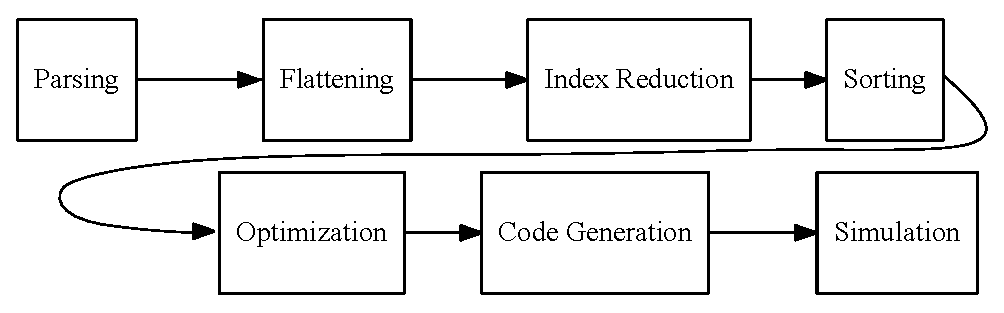
\includegraphics[scale=0.8]{pipeline} 
      \label{fig:proceso}
    \end{figure}
\end{frame}



\begin{frame}[fragile]
\frametitle{Simulación de Modelos Grandes} 
\begin{block}{Problemas}
Expandir las variables y ecuaciones vectorizadas implica un alto costo computacional en las siguientes etapas de compilación. \\
Imposibilidad de trabajar con sistemas de grandes dimensiones.
\end{block} 
\pause
\begin{block}{Objetivos}
Algoritmo de aplanado con costo computacional constante con respecto a la dimensionalidad (cantidad de variables) del modelo. \\
Mantener las definiciones de arreglos y ecuaciones \textit{for} durante toda la etapa de compilación.
\end{block} 
\end{frame}

\section{Algoritmo de aplanado}

\begin{frame}[fragile]
\frametitle{Modelo aplanado} 
\begin{block}{Modelo aplanado}
\begin{enumerate}
\item Modelo monolítico.
\item Carencias de clases.
\item Variables de tipo básicos.
\item No posee ecuaciones \textit{connect}.
\end{enumerate}
\end{block}
\end{frame}


\begin{frame}[fragile]
\frametitle{Algoritmo de aplanado} 
Esta dividido en dos etapas:
\begin{block}{Reducción de composiciones}
\begin{enumerate}
\item Expansión de herencia.
\item Simplificación de tipos.
\item Aplicación de modificaciones.
\item Reducción de instancias. 
\end{enumerate}
\end{block}

\begin{block}{Resolución de conexiones}
Descomposición de ecuaciones \textit{connect} en ecuaciones simples.
\end{block}
\end{frame}

\begin{frame}[fragile]
\frametitle{Algoritmo de aplanado} 
\begin{center}
\huge Reducción de composiciones
\end{center}
\end{frame}

\begin{frame}[fragile]
\frametitle{Algoritmo de Aplanado - Reducción de composiciones} 
\begin{lstlisting}[style=base,basicstyle=\scriptsize]
Flat(C):
    @2Expand(C);@
    foreach v in Variables(C):
        t = @2ResolveType(v)@;
        if isBasic(t) then 
            ChangeType(v,t);
        else if isClass(t) AND NOT isConnector(t) then
            @2ApplyModification(C,t,Modification(v));@
            Flat(t);
            @2RemoveComposition(C,t);@  
            if isConnector(t) then
                ChangeType(v,t);
            else
                Remove(t);
            end if;     
        end if;     
    end foreach;    
    foreach e in Equations(C):  
        @2ChangeVarName(e);@     
\end{lstlisting}
\end{frame}

\begin{frame}[fragile]
\frametitle{Expansión de herencias de clases} 

\begin{block} {}
La clase hijo hereda las variables y ecuaciones del padre.
\end{block}

\pause 
\begin{columns} 
\column[t]{.5\textwidth}   
\begin{lstlisting}[style=base,basicstyle=\scriptsize]
model OnePort
    Pin p;
    Pin n;
    Real v;
    Real i;
equation
    v = p.v - n.v;
    i = p.i;
    i = -n.i;
end OnePort;
model Capacitor
    extends OnePort;
    parameter Real C = 1;
equation
    C * der(v) = i;
end Capacitor;
\end{lstlisting} 
\pause
\column[t]{.5\textwidth}  
\begin{lstlisting}[style=base,basicstyle=\scriptsize]
model Capacitor 
    @2Pin p;@2
    @2Pin n;@
    @2Real v;@
    @2Real i;@2
    parameter Real C = 1;
equation
    @2v = p.v - n.v;@
    @2i = p.i;@
    @2i = -n.i;@
    C * der(v) = i;
end Capacitor;
\end{lstlisting}
\end{columns}
\end{frame}


\begin{frame}[fragile]
\frametitle{Simplificación de tipos - ResolveType} 
\begin{block}{}
Determina el tipo real de una variable y sus características: 
\begin{itemize}
    \item Prefijos de Tipos.
    \item Definición de Arreglos. 
    \item Presencia de modificaciones.
\end{itemize}
\end{block}
\pause
\begin{lstlisting}[style=base,literate={=}{$\leftarrow{}$}{1}{==}{$={}$}{1},escapechar=|,basicstyle=\scriptsize]
package Circuits |\only<3->{\color{blue}$\leftarrow$}|
    @4model Capacitor@
        extends OnePort;
        parameter Real C = 1;
    equation
        C * der(v) = i;
    end Capacitor;
    
    model LC_circuit |\only<2>{\color{blue}$\leftarrow$}|
        @Capacitor cap(v(start = 1));@
        inductor ind(L = 2);
        Pin p1,p2,p3;
    equation
        ...
    end LC_circuit;
end Circuits;
\end{lstlisting}
\end{frame}


\begin{frame}[fragile]
\frametitle{Aplicación de modificaciones - ApplyModification} 
\begin{block}{}
\begin{enumerate}
\item Expandir la clase.
\item Agregar las modificaciones a la variable correspondiente.
\end{enumerate}
\end{block}
\pause
Capacitor c (C=5,v(start=2))
\pause
\begin{columns} 
\column[t]{.5\textwidth}  
\begin{lstlisting}[style=base,basicstyle=\scriptsize]
model Capacitor 
    Pin p;
    Pin n;
    Real v;
    Real i;
    parameter Real C = 1;
equation
    v = p.v - n.v;
    i = p.i;
    i = -n.i;
    C * der(v) = i;
end Capacitor;
\end{lstlisting}
\column[t]{.5\textwidth}  
\begin{lstlisting}[style=base,basicstyle=\scriptsize]
model Capacitor 
    Pin p;
    Pin n;
    Real v @(start=2)@;
    Real i;
    parameter Real @C = 5@;
equation
    v = p.v - n.v;
    i = p.i;
    i = -n.i;
    C * der(v) = i;
end Capacitor;
\end{lstlisting}
\end{columns}
\end{frame}

\begin{frame}[fragile]
\frametitle{Reducción de instancias - RemoveComposition} 
\begin{block}{RemoveComposition}
\begin{enumerate}
\item Reemplaza las instancias de clases (previamente aplanada).
\item Añade las variables y ecuaciones internas.
\item Renombrar las variables añadidas.
\item Si la instancia está vectorizada: 
    \begin{enumerate}
    \item Agrega las variables vectorizadas.
    \item Encapsulamos las ecuaciones dentro de una ecuación \textit{for}.
    \end{enumerate} 
\end{enumerate}
\end{block}
\end{frame}

\begin{frame}[fragile,t]
\frametitle{RemoveComposition} 
\begin{block}{Variables}
\begin{enumerate}
\item Agrega un prefijo al nombre de las variables: "nombreInstancia\_".
\item Mantiene los prefijos de tipos de las  variable. 
\item Mantiene las definiciones de arreglos y agrega nuevas si la instancia lo está.   
\end{enumerate}
\end{block}

\begin{block}{Ecuaciones}
\begin{enumerate}
\item Renombra las variables que correspondan.
\item Reemplaza el operador ''.'' por guiónes.
\item Encapsula las ecuaciones en un \textit{for} si la instancia esta vectorizada.
\end{enumerate}
\end{block}
\end{frame}

\begin{frame}[fragile]
\frametitle{Algoritmo de Aplanado - Reducción de composiciones} 
\begin{lstlisting}[style=base,basicstyle=\scriptsize]
Flat(C):
    @2Expand(C);@
    foreach v in Variables(C):
        t = @2ResolveType(v)@;
        if isBasic(t) then 
            ChangeType(v,t);
        else if isClass(t) AND NOT isConnector(t) then
            @2ApplyModification(C,t,Modification(v));@
            Flat(t);
            @2RemoveComposition(C,t);@  
            if isConnector(t) then
                ChangeType(v,t);
            else
                Remove(t);
            end if;     
        end if;     
    end foreach;    
    foreach e in Equations(C):  
        @2ChangeVarName(e);@     
\end{lstlisting}
\end{frame}

\begin{frame}[fragile]
\frametitle{RemoveComposition: Ejemplos}
\begin{columns} 
\column[t]{7cm}  
\begin{lstlisting}[style=base,basicstyle=\scriptsize]
package Circuits
    @2model LC_circuit@
        Pin p1,p2,p3;
    equation
        p1.v = p2.v;
        p2.v = p3.v;
    end LC_circuit;
    
    model LC_line
        constant Integer N = 10;
        LC_circuit lc[N];
        ground gr;
    equation
        connect(lc[N].p1,lc[N].p2)      
        for i in 1:N - 1 loop
            connect(lc[i + 1].p3,lc[i].p2);
        end for;
        for i in 1:N loop
            connect(gr.p,lc[i].p1);
        end for;
    end LC_line;
end Circuits;
\end{lstlisting}

\column[t]{7cm}  
\begin{lstlisting}[style=base]
package Circuits
    model LC_circuit
        Pin p1,p2,p3;
        flow Real p1_i,p2_i,p3_i;
        Real p1_v,p2_v,p3_v;
    equation
        p1_v = p2_v;
        p2_v = p3_v;
    end LC_circuit;
end Circuits;
\end{lstlisting}
\end{columns}
\end{frame}

\begin{frame}[fragile]
\frametitle{RemoveComposition: Ejemplos}
\begin{columns} 
\column[t]{7cm}  
\begin{lstlisting}[style=base,basicstyle=\scriptsize]
    model LC_circuit
        Pin p1,p2,p3;
        flow Real p1_i,p2_i,p3_i;
        Real p1_v,p2_v,p3_v;
    equation
        p1_v = p2_v;
        p2_v = p3_v;
    end LC_circuit;
    
    model LC_line
        constant Integer N = 10;
        @2LC_circuit lc[N];@
        ground gr;
    equation
        connect(lc[N].p1,lc[N].p2)      
        for i in 1:N - 1 loop
            connect(lc[i + 1].p3,lc[i].p2);
        end for;
        for i in 1:N loop
            connect(gr.p,lc[i].p1);
        end for;
    end LC_line;
\end{lstlisting}

\column[t]{8cm}  
\begin{lstlisting}[style=base,basicstyle=\scriptsize]
package Circuits
    model LC_line
        constant Integer N = 10;
        Pin p1[N],p2[N],p3[N];
        flow Real lc_p1_i[N],lc_p2_i[N],lc_p3_i[N];
        Real lc_p1_v[N],lc_p2_v[N],lc_p3_v[N];
        ground gr;
    equation
        for i in 1:N - 1 loop
            p1_v[N] = p2_v[N];
            p2_v[N] = p3_v[N];
        end for;
        connect(lc_p1[N],lc_p2[N])      
        for i in 1:N - 1 loop
            connect(lc_p3[i + 1],lc_p2[i]);
        end for;
        for i in 1:N loop
            connect(gr_p[i],lc_p1[i]);
        end for;
    end LC_line;
end Circuits;
\end{lstlisting}
\end{columns}
\end{frame}



\begin{frame}[fragile]
\frametitle{Algoritmo de aplanado} 
\begin{center}
\huge Resolución de conexiones
\end{center}
\end{frame}

\begin{frame}[fragile]
\frametitle{Resolución de conexiones} 
\begin{block}{En un principio}
\begin{enumerate}
\item Expandir las ecuaciones \textit{for}.
\item Generar de un grafo a partir de las ecuaciones \textit{connects}.
\item Determinar las componentes conexas del grafo generado.
\item Generación de ecuaciones a partir de las componentes conexas.
\end{enumerate}
\end{block}

\pause
\begin{block}{Proponemos}
\begin{enumerate}
\item Grafo bipartito cuyos nodos y aristas están etiquetadas según las ecuaciones. \\Grafo Vectorizado.
\item Búsqueda en profundida modificada para determinar las componentes conexas.    
\item Generación de ecuaciones a partir de las componentes conexas.
\end{enumerate}
\end{block}

\end{frame}

\begin{frame}{fragile}
\frametitle{Grafo Vectorizado}
\begin{enumerate}
\setlength\itemsep{1em}
\item Agregamos un nodo por cada variable de la ecuación.
\item Agregamos un nodo que representa a la ecuación \textit{connect}.
\item Si la ecuación estaba dentro de un \textit{for}, etiquetamos el nodo \textit{connect} con el rango de iteraci\'on. 
\item Agregamos dos aristas, entre cada variable y el nodo que representa al \textit{connect}.
\item Por cada arista, si la variable asociada tiene un índice de acceso, agregamos esa referencia a la arista. 
\end{enumerate}
\end{frame}

\begin{frame}[fragile]
\frametitle{Grafo Bipartito: Ejemplo}
\begin{columns} 
\column[t]{7cm}  
\begin{lstlisting}[style=base]
connect(lc_p1[N],lc_p2[N])     
 
for i in 1:N - 1 loop
    connect(lc_p3[i + 1],lc_p2[i]);
end for;

for i in 1:N loop
    connect(gr_p[i],lc_p1[i]);
end for;
\end{lstlisting}

\column[t]{7cm}  

\begin{tikzpicture}[>=stealth',shorten >=1pt,auto, node distance = 1.5cm,
                    thick,main node/.style={circle,draw,font=\sffamily\bfseries}]
 
  \node[main node] (4)  {gr\_p};
  \node[main node] (1) [below of=4] {lc\_p1};
  \node[main node] (2) [below of=1] {lc\_p2};
  \node[main node] (3) [below of=2] {lc\_p3};
  
  
  \node[main node] (7) [right of = 4, xshift=3cm]  {1:N};
  \node[main node] (5) [below of=7] {\{\}};
  \node[main node] (6) [below of=5]  {1:N-1};
    
    
  \path[every node/.style={font=\sffamily\small}]   
    (1) edge node [left,near start,above] {N} (5)
        edge node[left,very near start,above] {i} (7)
    (2) edge node [left,pos = 0.05,above] {N} (5)
        edge node[left,very near start,below] {i} (6)  
    (3) edge node [left,near start,above] {i + 1} (6)    
    (4) edge node [left,near start,above] {i} (7);
\end{tikzpicture}
\end{columns}
\end{frame}

\begin{frame}{fragile}
\frametitle{Determinación de componentes conexas}
\begin{itemize}
\setlength\itemsep{1em}
\item Búsqueda en profundida sobre el grafo. 
\item Cada visita a un nodo depende de la metadata del grafo.
\item Múltiples visitas a un mismo nodo. 
\item Mantenemos referencia del intervalo de acceso al nodo. 
\item Visitamos un nodo si hay intersección entre intervalos.
\item Podamos parte de la arista al visitar un nodo.
\item Terminamos cuando no hay más intersección con otros nodos.
\end{itemize}
\end{frame}


\begin{frame}[fragile]
\frametitle{Determinación de componentes conexas}
\begin{columns} 
\column[t]{7cm}  
  \newcommand*\nstart{} 
  \newcommand*\none{}
  \newcommand*\ntwo{}
  \newcommand*\nfive{}
  \newcommand*\nsixe{}
  \newcommand*\nocho{}
  \only<1-2>{\renewcommand*\nstart{green}}
  \only<2->{\renewcommand*\none{blue}}
  \only<3-5>{\renewcommand*\ntwo{green}}
  \only<5->{\renewcommand*\nfive{blue}}
  \only<6->{\renewcommand*\nsixe{green}}
  \only<8>{\renewcommand*\nocho{blue}}

\begin{tikzpicture}[>=stealth',shorten >=1pt,auto, node distance = 1.5cm,
                    thick,main node/.style={circle,draw,font=\sffamily\bfseries}]  
                    
  \node[main node, \nstart] (4)  {gr\_p};
  \node[main node,\ntwo] (1) [below of=4]{lc\_p1};
  \node[main node,\nsixe] (2) [below of=1] {lc\_p2};
  \node[main node] (3) [below of=2] {lc\_p3};
  
  
  \node[main node] (7) [right of = 4,xshift=3cm]  {1:N};
  \node[main node] (5) [below of=7 ] {\{\}};
  \node[main node] (6) [below of=5]  {1:N-1};
    
    
  \path<1-6>[every node/.style={font=\sffamily\small}]  
    (1) edge[\nfive] node [left,near start,above] {N} (5)
    (2) edge[\nfive] node [left,pos = 0.05,above] {N} (5);
    
   \path[every node/.style={font=\sffamily\small}]    
     (2)   edge[\nocho] node[left,very near start,below] {i} (6)  
    (3) edge node [left,near start,above] {i + 1} (6);
    
   \path<1-3>[every node/.style={font=\sffamily\small}]     
        (1) edge[\none] node[left,very near start,above] {i} (7)    
        (4) edge[\none] node [left,near start,above] {i} (7);
        
\end{tikzpicture}

\column[t]{8cm}  
\begin{enumerate}
\item Arrancamos en \textit{gr\_p}.
\item<2-> Existe único camino y tiene intervalo 1:N.
\item<3-> Visitamos \textit{lc\_p1} con intervalo 1:N.
\item<4-> Podamos el grafo.
\item<5-> Existe un camino con índice N.
\item<6-> Visitamos \textit{lc\_p2} con índice N.
\item<7-> Podamos el grafo.
\item<8-> $N \cap 1:N-1 = \{\}$. \\
          No hay más nodos para buscar.

\end{enumerate}
\end{columns}
\end{frame}

\begin{frame}[fragile]
\frametitle{Determinación de componentes conexas}
\begin{columns} 
\column[t]{7cm}  

  \newcommand*\nstart{} 
  \newcommand*\none{} 
  \newcommand*\ntwo{} 
  \only<1>{\renewcommand*\nstart{green}}
  \only<2-3>{\renewcommand*\none{green}} 
  \only<4->{\renewcommand*\ntwo{green}} 

\begin{tikzpicture}[>=stealth',shorten >=1pt,auto, node distance = 1.5cm,
                    thick,main node/.style={circle,draw,font=\sffamily\bfseries}]  
  
  \node[main node,\ntwo] (4)  {gr\_p};
  \node[main node,\none] (1) [below of=4]{lc\_p1};
  \node[main node,\nstart] (2) [below of=1] {lc\_p2};
  \node[main node] (3) [below of=2] {lc\_p3};
  
  
  \node[main node] (7) [right of = 4,xshift=3cm]  {1:N};
  \node[main node] (5) [below of=7] {\{\}};
  \node[main node] (6) [below of=5]  {1:N-1};
     
    
   \path[every node/.style={font=\sffamily\small}]    
    (2) edge node[left,very near start,below] {i} (6)  
    (3) edge node [left,near start,above] {i + 1} (6); 
        
\end{tikzpicture}

\column[t]{8cm}  
\begin{enumerate}
\setlength\itemsep{2em}
\item En \textit{lc\_p2} la solución es:    
    \begin{itemize}
    \item $\langle \ \textit{lc\_p2[N]} \ \rangle$. 
    \end{itemize}

\item<2-> En \textit{lc\_p1} hubo una partición de intervalos:
    \begin{itemize}
    \item $1:N-1$ \only<3->{$\rightarrow \  \langle \textit{lc\_p1[i]} \  \rangle$ en $1:N-1$ }
    \item $N$     \only<3->{$\rightarrow \  \langle \textit{lc\_p1[N]},\ \textit{lc\_p2[N]} \  \rangle$ }
    \end{itemize}
    
\item<4-> En \textit{gr\_p} las soluciones finales son:
    \begin{itemize}
    \item $\langle \  \textit{gr\_p[i]},\ \textit{lc\_p1[i]} \  \rangle$ en $1:N-1$
    \item $\langle \  \textit{gr\_p[N]},\ \textit{lc\_p1[N]},\ \textit{lc\_p2[N]} \  \rangle$  
    \end{itemize}
    
\end{enumerate}
\end{columns}
\end{frame}



\begin{frame}{fragile}
\frametitle{Generación de ecuaciones}
\begin{itemize}
\setlength\itemsep{1em}
\item Cada componente conexa determina un conjunto de ecuaciones.
\item Determinar el tipo de conector usado.
\item Las variables de potencial deben quedar igualadas entre sí.
\item Las variables de flujo deben sumar cero. 
\end{itemize}
\end{frame}

\begin{frame}[fragile]
\frametitle{Generación de ecuaciones} 
\begin{itemize}
\item $\langle \ \textit{gr\_p[i]},\ \textit{lc\_p1[i]} \ \rangle$ en $1:N-1$. \\
\vspace{1em}
\begin{lstlisting}[style=base]
    @2for i in 1:N - 1 loop@
        gr_p_v[i] = lc_p1_v[i];
        gr_p_i[i] + lc_p1_i[i] = 0;
    @2end for;@
\end{lstlisting}

\pause
\item $\langle \ \textit{gr\_p[N]},\ \textit{lc\_p1[N]},\ \textit{lc\_p2[N]} \ \rangle$ . \\
\vspace{1em}
\begin{lstlisting}[style=base]
    gr_p_v[N] = lc_p1_v[N];  
    gr_p_v[N] = lc_p2_v[N];
    gr_p_i[N] + lc_p2_i[N] + lc_p2_i[N] = 0;
\end{lstlisting}
\end{itemize}
\end{frame}

\section{Implementación y Comparaciones}

\begin{frame}[fragile]
\frametitle{Implementación y Comparaciones} 
\begin{block}{Algoritmo de Aplanado}
\begin{enumerate}
\item Implementados en C++.
\item Uso de las estructuras de datos de la librería Boost (AST, Árboles, Parser).
\item Pertenece al proyecto ModelicaCC  \footnote{http://sourceforge.net/projects/modelicacc/}, que contiene diversas herramientas para compilar los modelos y simularlos. 
\item Realizamos pruebas de performance en varios ejemplos variando el parámetro N.
\end{enumerate}
\end{block}
\end{frame}

\begin{frame}[fragile]
\frametitle{Comparaciones con otros algoritmos}
\begin{table}[ht]
 \centering 
	\begin{tabular}{ | c | c | c | c | c |}
	\hline
	   N  & \multicolumn{2}{|c|}{OpenModelica} & \multicolumn{2}{|c|}{ModelicaCC} \\ \cline{2-5}
				& Tiempo(seg)	& Tamaño(bytes)	& Tiempo(seg)	& Tamaño(bytes) \\ \hline
	   10    	& 3.792  		& 33.212		& 0.048 		& 3.708		\\ \hline
	   100   	& 5.632   	 	& 302.374 		& 0.052    		& 3.723 		\\ \hline
	   500   	& 19.440 		& 818.439 		& 0.044    		& 3.725 		\\ \hline
	   1000  	& 51.628 		& 3.048.164	 	& 0.052	 		& 3.738		\\ \hline
	   3000  	& 393.452 		& 9.272.336		& 0.044	 		& 3.740		\\ \hline
	   5000  	& 1107.732 		& 15.496.336	& 0.052	 		& 3.740		\\ \hline
	   10000 	& Error			& Error			& 0.058			& 3.753		\\ \hline
	\end{tabular}	 
	\caption{Tiempos de aplanado variando $N$ para el modelo LC\_line }
\end{table}
\end{frame}

\section{Conclusiones y Trabajo a Futuro}
\begin{frame}
\frametitle{Conclusiones}
\begin{itemize}
 \item Desarrollamos un algoritmo de aplanado que preserva la vectorización del modelo.
 \item Desarrollamos un métodos para encontrar las componente conexas dentro de un grafo bipartito vectorizado.
 \item Implementamos ambos algoritmos en C++ dentro de la herramienta ModelicaCC.
 \item Realizamos pruebas tanto de ejemplos simples como de ejemplos vectoriales, concluyendo que las transformaciones aplicadas por la herramienta desarrollada llegaban al resultado correcto.
 \item Comparamos nuestra implementación del algoritmo de aplanado con la de la herramienta OpenModelica para distintos tamaños de modelos vectorizados, obteniendo un costo constante en función de la cantidad de variables del modelo. 
 
\end{itemize}
\end{frame}


\begin{frame}
\frametitle{Trabajo a Futuro}
\begin{itemize}
\item Realizar pruebas con nuevos ejemplos para soportar aun más las características de Modelica.

\item Adaptar el algoritmo de resolución de ecuaciones \textit{connect} para resolver anidaciones de dos o más ecuaciones \textit{for}.

\item Aplicar un caché de modelos aplanados con el objetivo de reducir a uno la cantidad de veces que aplanamos una misma clase.  

\item Estudiar la posibilidad de paralelizar el aplanado de clases.  
  
\end{itemize}
\end{frame}

\begin{frame}[fragile]
\frametitle{Fin} 
\begin{center}
\huge ¡Muchas Gracias! \\
\LARGE ¿Preguntas?
\end{center}
\end{frame}




\end{document}
    
